\subsection{MMM kernels generation}
\label{sec:contributions}
It is clear that the importance budgets implied in training LLMs is no afordable in a age where known computer science laws are being rstes such moore law, dennard, dark silicon era.

Which explains the heavy need for specialization, specialized cirtuits to explore the emerging float format in the cotext of mmm units. which is possible with the fast evolution of open source EDA tools~\cite{OpenROAD,us_osda}.

Figure~\ref{weight_distribution} puts together the distribution of the weights dynamic range alongside with the computer format we evaluate.
The evaluations comprise the computer formats of the figure with different Systolic Array sizes with five PDKs (GF180, SKy130hd, Sky130hs, nangate45, ASAP7) which allow to verify scalability of designs without the use of manual scaling.

2 variations of accum per arith, very important as computing is less expensive than communictaion, we can add some complexity in the chip to leverage data movemenrt by taking int oaccount he sequential nature of mmm and dot products maximizing entropy.

\begin{figure}[b]
\centering
	\vspace{-0.5cm}
	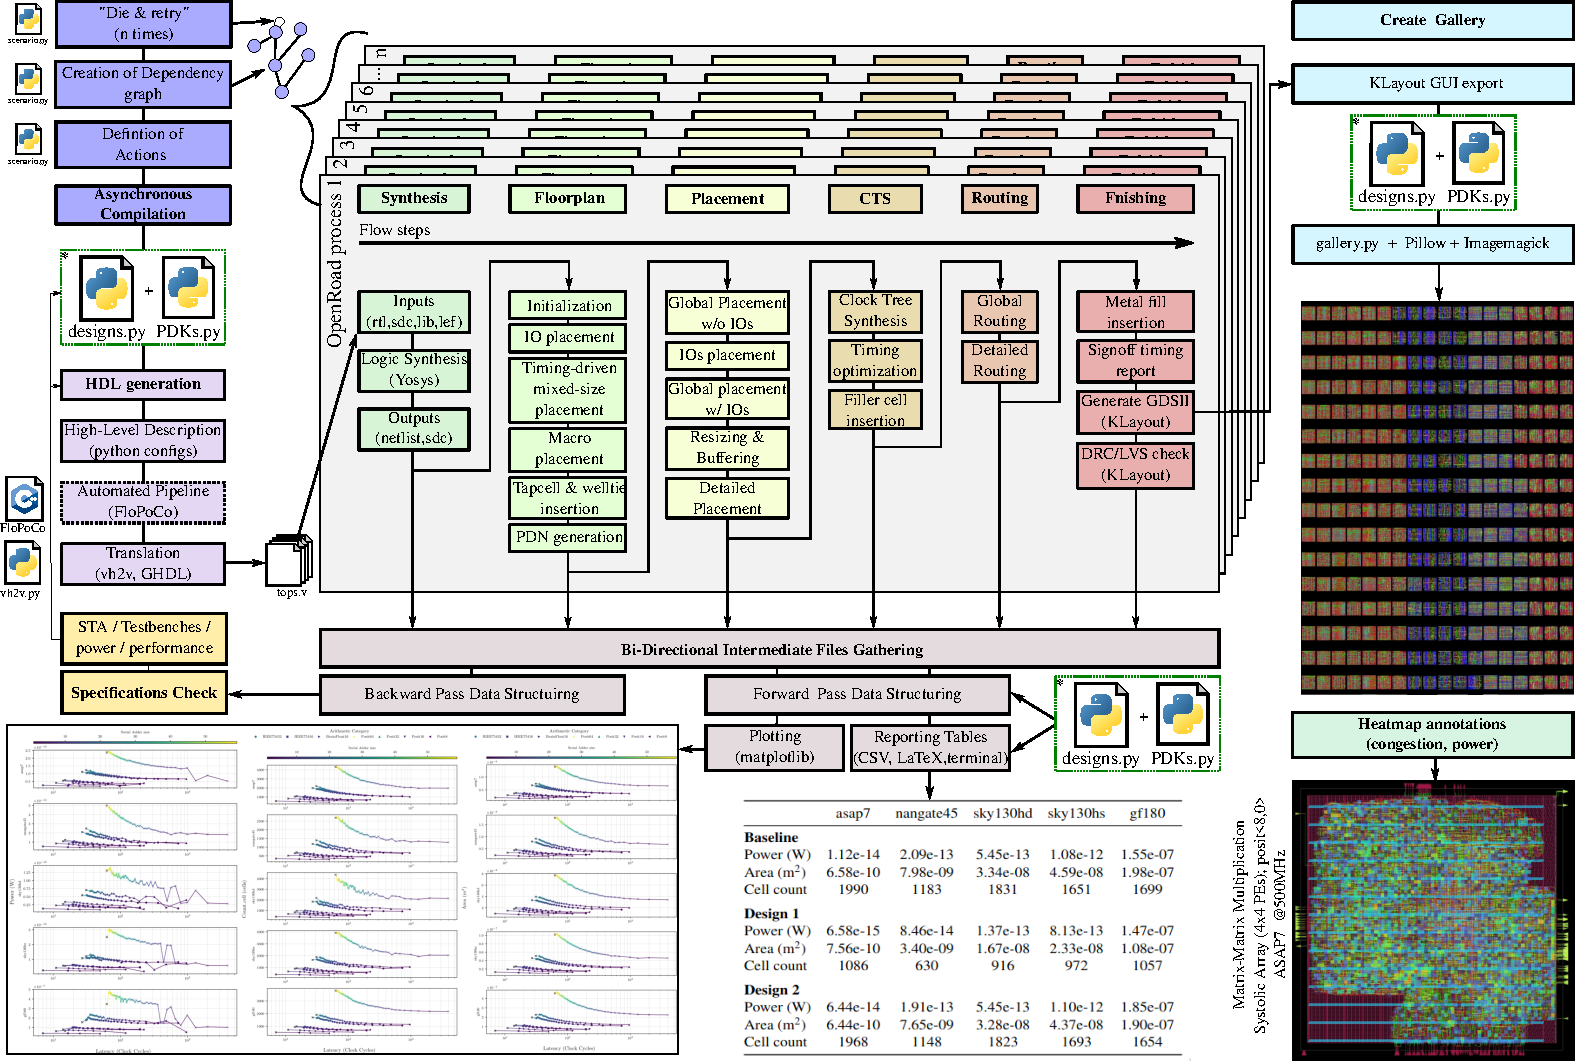
\includegraphics[width=\columnwidth]{./figures/SUF.pdf}
	\vspace{-0.5cm}
	\caption{Schematic Overview SUF: Centralized Management of Asynchronous OpenROAD Forks, Derived from Dependency Task Graphs. This illustration also encapsulates the extended capabilities ranging from Code Generation without manual RTL Writing to Advanced Plotting and Visualization Features.}
	\label{fig:suf}
\end{figure}

\subsection{Chips}
\begin{figure}[H]
\centering
	\vspace{-0.5cm}
	\includegraphics[width=0.5\columnwidth]{./figures/SA_8x8_e4m3_rulers_congestion.png}
	\vspace{-0.5cm}
	\caption{e4m3 cogestion routed highlighted beta 8x8}
	\label{fig:focus on e4m3}
\end{figure}

\begin{figure}[H]
\centering
	\vspace{-0.5cm}
	\includegraphics[width=\columnwidth]{./figures/systolic_arrays.png}
	\vspace{-0.5cm}
	\caption{All generated arrays}
	\label{fig:all_arrays}
\end{figure}


\subsection{Early Results}

The evaluation of 14 design entries, with posit 4 beta not working finished in two hours yielding a total of xx chips.
Figure~\ref{fig:power_vs_area} shows depicts power and area accross 5 process nodes.
\begin{figure}[t]
\centering
	\vspace{-0.5cm}
	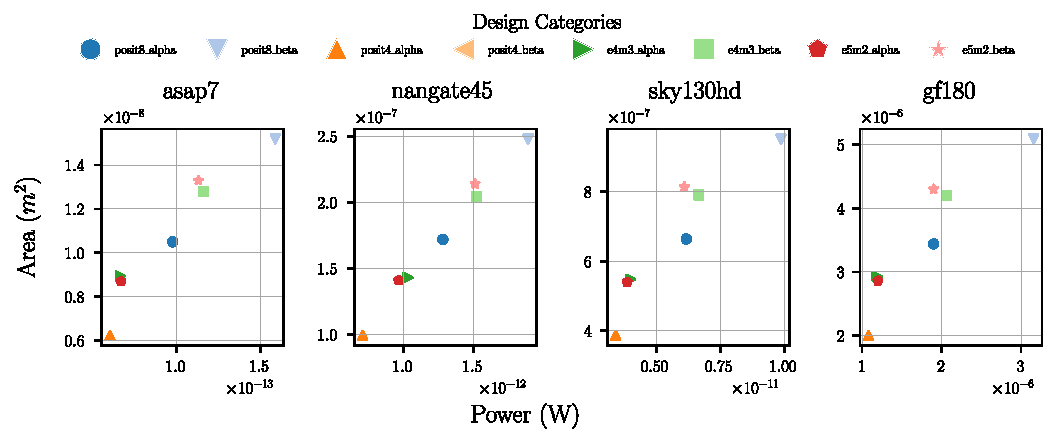
\includegraphics[width=\columnwidth]{./figures/power_vs_area_comparison.pdf}
	\vspace{-0.5cm}
	\caption{Area vs. Power}
	\label{fig:power_vs_area}
\end{figure}

